%!TEX root = ..\..\main.tex

\section{Methode}
\label{Methode}
In den nächsten Abschnitten wird im Detail auf die RDF~\cite{HartleyRadDist} und die LMA~\cite{LevMarquardt} eingegangen. Die RDF beschreibt das Verhalten der Linsenverzerrung und mit Hilfe der LMA können die entsprechenden Verzerrungskoeffizienten aus korrespondierenden Punktepaaren  approximiert werden. Diese Paare beinhalten stets einen Punkt in der Welt und den entsprechenden Bildpunkt auf den er abgebildet wird.

\subsection{Radial Distance Function (RDF)}
\label{sec:RDF}
\todo[inline, color=yellow]{Vera}
Die oben beschriebene kissenförmige Linsenverzerrung ist demzufolge konvex und strikt symmetrisch um die optische Achse~\cite{WengRadDist}. Es kann daher vorausgesetzt werden, dass der Bildhauptpunkt $c= \begin{pmatrix}
c_x & c_y
\end{pmatrix}^T$ im Zentrum der radialen Verzerrung liegt. In diesem Fall kann die Linsenverzerrung, wie in Formel~\ref{equ:BasicModel} moduliert werden. Hier werden die unverzerrten und linearen Bildkoordinaten als $u= \begin{pmatrix}
u_x & u_y
\end{pmatrix}^T$ und die verzerrten Bildpunkte als $d= \begin{pmatrix}
d_x & d_y
\end{pmatrix}^T$ bezeichnet. $L(r)$ definiert die Linsenfunktion des Systems und ist abhängig vom Abstand $r$.

\begin{equation}
\label{equ:BasicModel}
\begin{pmatrix}
d_x \\
d_y\\
\end{pmatrix} =
L(r)
\begin{pmatrix}
u_x-c_x\\
u_y -c_y\\
\end{pmatrix}
\end{equation}

Der Abstand $r$ ist definiert als euklidischer Abstand vom Zentrum $c$, wie in Formel~\ref{equ:Abstand} aufgeführt. Aus nummerischen Gründen wird für die Approximation die Form $r^2$ verwendet, welche den Rundungsfehler und den Rechenaufwand minimiert. 

\begin{equation}
\label{equ:Abstand}
r = \sqrt{u_x^2+u_y^2}
\end{equation}

 Für die Linsenfunktion gilt $L(c)=1$, da der Betrag der Verzerrung mit zunehmenden Abstand größer wird. $L(r)$ ist für alle weiteren Bildpunkte unbekannt. Daher wird $L(r)$ um $r=0$ mit einer Taylorreihe approximiert (vgl. Formel~\ref{equ:Taylor}). 
 
 \begin{equation}
 \label{equ:Taylor}
 L(r)=1+\kappa_1*r+\kappa_2*r^2+\kappa_3*r^4 + \dots
 \end{equation}

Mit den Koeffizienten $\kappa_1, \kappa_2, \kappa_3, \dots$ kann die radiale Verzerrung des Bildes korrigiert werden und ausgehend von einer quadratischen Approximation gibt sich anhand Formel~\ref{equ:Taylor} die RDF für $u_x$ und $u_y$ mit Formel~\ref{equ:RDF}~\cite{WangRaddist}.

\begin{equation}
\label{equ:RDF}
\begin{split}
u_x = d_x*(1+\kappa_1*r+\kappa_2*r^2+\kappa_3*r^4 + \dots) + c_x\\
u_y = d_y*(1+\kappa_1*r+\kappa_2*r^2+\kappa_3*r^4 + \dots) + c_y
\end{split}
\end{equation}

Die unbekannten Koeffizienten $\kappa_1, \kappa_2, \kappa_3, \dots$ können mit einer nicht-linearen Ausgleichsrechnung approximiert werden indem das Minimierungsproblem mit der RDF moduliert wird. Ein effizientes Verfahren zur Approximierung der Koeffizienten ist die bekannte LMA~\cite{LevMarquardt}.
\subsection{Levenberg-Marquard-Approximation}
\todo[inline, color=yellow]{Vera}
Die \textit{Methode der kleinsten Quadrate} von Gauß ist ein bekanntes Verfahren, welches die unbekannten Parameter $\alpha$ von überbestimmten Systemen aus linearen oder nichtlinearen Gleichungen annähert. Diese Systeme werden in der Regel aus Wertepaaren moduliert, welche im Voraus gemessen und bestimmt wurden. Der Messwert wird im folgenden als $y$ und der als ideale angenommene Wert $t$ bezeichnet.
Im Fall der einer radialen Entzerrung sollte für die Anzahl der Wertepaare $M>3$ sein um eine gute Näherung der Parameter beziehungsweise Koeffizienten zu ermitteln.
Es handelt sich somit um ein überbestimmtes System, welches nicht exakt lösbar ist. In diesem Fall kann nur verlangt werden, dass die Abweichungen und Residuen minimal sind~\cite{schwarz2011numerische}. 

Für die \textit{Methode der kleinsten Quadrate} wird die euklidische Norm des Residuums $b-Ax$ minimiert~\cite{dahmen2008numerik} und das entsprechende lineare Ausgleichsproblem wird wie in Formel~\ref{equ:LinAusgleich} formuliert. Hier gibt $N$ die Anzahl der Parameter und $M$ die Anzahl der gemessenen Wertepaare an. Die Matrix $A$ enthält die gesuchten Parameter $a_{i,j=1}$ und der Vektor $b$ alle gemessenen Werte.
\begin{equation}
\label{equ:LinAusgleich}
\begin{aligned}
& ||Ax^*-b||_2 = \min_{x\in \mathbb{R}^N} ||Ax-b||_2\\
& mit\ A\in \mathbb{R}^{M\times N}\ und\ b\in \mathbb{R}^{N}
\end{aligned}
\end{equation}

Lineare Ausgleichsprobleme können mit einer Vielzahl an verschieden Verfahren gelöst werden, wie zum Beispiel einer \textit{Cholesky}- beziehungsweise QR-Zerlegung oder der Singulärwertzerlegung.
Doch diese Verfahren können nur dann angewendet werden, wenn der Messwert $y$ von allen Parametern linear abhängig ist. Ist dies nicht gegeben, handelt es nicht um ein nichtlineares Ausgleichsproblem, wie bei der RDF (vgl. Formel~\ref{equ:RDF}). Zur Lösung dieser Art von Ausgleichsverfahren werden in der Praxis das \textit{Gauß-Newton-Verfahren} (GNV) und die LMA angwendet. Letzteres ist eine effizientere Weiterentwicklung des GNV und eine geeignete Wahl um die Koeffizienten $\kappa$ der RDF zu approximieren.

Im Sinne der \textit{Methode der kleinsten Quadrate} lässt sich das nichtlineare Ausgleichsproblem wie in Formel \ref{equ:LinAusgleich} definieren~\cite{schwarz2011numerische}. $F(x)$ ist definiert als Abbildung $F: \mathbb{R}^N \arrowvert \mathbb{R}^M$ und $F_i()x:= y(t_i,x)-b_i\ mit\ i= 1,\dots,M$. 

\begin{equation}
\label{equ:LinAusgleich}
\begin{aligned}
||F(x^*)||_2 =& \min_{x\in \mathbb{R}^N} ||F(x)||_2\\
\phi(x^*)=& \min_{x\in \mathbb{R}^N} ||\phi(x)||_2 = \frac{1}{2}||F(x)||_2^2 = \frac{1}{2}F(x)^TF(x)
\end{aligned}
\end{equation}

Die iterative Lösung des GNV basiert auf der grundlegenden Annahme, dass der Gradient $\Delta\phi(x)$ an einem kritischen Punkt Null sein muss. Darum wird angenommen, dass der Gradient $\Delta\phi(x^*)$ ein lokales Minimum ist. Weiter ergibt sich durch Nachrechnen für $\Delta\phi(x)$ die Gleichung~\ref{equ:GradPhi}, wobei $F'(x) \in \mathbb{R}^{M \times N}$ die Jacobi-Matrix von $F$ ist und für das iterative GNV benötigt wird~\cite{dahmen2008numerik}.


\begin{equation}
\label{equ:GradPhi}
\Delta\phi(x)=F'(x)^TF(x)
\end{equation}

Das GNV versucht die Lösung $x$ mit Hilfe von geeigneten linearen Problemen unter der Voraussetzung eines geeigneten Startwerts $x_0$ anzunähern. Deshalb wird $F$ zunächst in eine lineare Approximation mittel Taylorentwicklung zerlegt und führt zu der Problemdefinition in Formel~\ref{equ:Newton}~\cite{LevMarquardt}. Während des iterativen Prozesses wird $x^k$ immer weiter an die gesuchte Lösung angenähert, in dem die Lösung des linearen Ausgleichsproblems $s^k$ nach jeder Iteration auf das aktuelle $x^k$ aufaddiert wird. Die Lösung $s^k$ kann bekannterweise mit der \textit{Cholesky}- oder QR-Zerlegung gelöst werden~\cite{schwarz2011numerische}.

\begin{equation}
\label{equ:Newton}
||F'(x^k)s^k+F(x^k)||_2 = \min_{s^k \in \mathbb{R}^N}||F'(x^k)s^k+F(x^k)||_2
\end{equation}

Das oben beschriebene Vorgehen wird wiederholt bis das Abbruchkriterium aus Formel~\ref{equ:Abbruchkriterium} erfüllt ist. Die Fehlertoleranz $\epsilon$ kann geeignet vom Nutzer vorgegeben werden.

\begin{equation}
\label{equ:Abbruchkriterium}
||F'(x^k)F(x^k)||_2 \leq \epsilon\\
\end{equation}

Problematisch wird ein Lösungsverfahren mit GNV, wenn $F$ keinen vollen Rang hat. In diesem Fall kann keine eindeutige Lösung approximiert werden. Dieses Problem umgeht die LMA in dem das Modell aus Formel~\ref{equ:Newton} durch den freiwählbaren Parameter $\mu>0$ in Formel~\ref{equ:Levenberg} erweitert wird. 

\begin{equation}
\label{equ:Levenberg}
||
\begin{pmatrix}
F'(x^k)\\\nu I\\
\end{pmatrix}
s^k+\begin{pmatrix}
F'(x^k)\\\emptyset\\
\end{pmatrix}||_2 = \min
\end{equation}

Mit einer geeignet großen Wahl von $\mu$ kann eine Korrektur von $s^k$ erreicht werden, welche eine deutliche Verbesserung in Richtung des lokalen Minimums bewirkt. Ein sehr großes $\mu$ verlangsamt die Konvergenz signifikant und mit einer sehr niedrigen Wahl kann unter Umständen keine Konvergenz gewährleistet werden. Aus diesem Grund wird das iterative Verfahren des GNV für die LMA um einen Zwischenschritt erweitert. Für jede Lösung $s^k$ wird getestet ob die Korrektur angemessen ist. Entspricht die ermittelte Korrektur nicht den Bedingungen wird $\mu$ entsprechend angepasst und $s^K$ erneut berechnet. Dieser Schritt wird solange iteriert bis die Bedingungen erfüllt sind und im nächsten Schritt mit der Berechnung von $x^{k+1}$ fortgeführt werden kann~\cite{dahmen2008numerik}. Als Abbruchkriterium für die LMA gilt auch Formel~\ref{equ:Abbruchkriterium}.

 

\section{System}
\label{sec:System}

In den folgenden Abschnitten wird auf das implementierte System eingegangen. Zunächst wird in Abschnitt~\ref{sec:Wertpaare} dargelegt wie Wertpaare und insbesondere die idealen Koordinaten des Punktrasters ermittelt wurden. Im Anschluss wird im Abschnitt~\ref{sec:Problem} das Problem der LMA moduliert und in Abschnitt~\ref{sec:Minimierung} die Initialisierung der LMA beschrieben. Zuletzt wird aufgezeigt wie das Java Plugin aufgebaut wurde und alle implementierten Funktionen erläutert.


\subsection{Ermittlung der Wertpaare}
\label{sec:Wertpaare}

UnwarpJ erzeugt in der \textit{Landmarks}-Datei die Wertepaare nicht in der Reihenfolge in der die Punkte gesetzt wurden, deswegen war es nicht möglich die Ziel-Koordinaten zur Laufzeit zu berechnen. Hierzu war es notwendig zuerst in das Ausgangsbild das optimale Gitter einzuzeichnen und danach die Punkt-Paare mit Hilfe von UnwarpJ zu setzen.

Dafür wurden in der Plugin-Klasse die Gitterparameter als Konstanten angelegt und das Zeichnen der Gitterpunkte in der Methode \texttt{compute\_draw\_optimal\_Grid()} (vgl. Abschnitt~\ref{sec:PluginKlassen}) realisiert.

Zur Berechnung der Ziel-Koordinaten wurden die folgenden Werte aus Tabelle \ref{tab:gitter_koordinaten_variablen} genutzt:

\begin{table}[H]
\centering
\begin{tabular}{|l|l|p{0.5\textwidth}|}
\hline
Variablen-Name & Wert & Funktion\\
\toprule[2px]
$dist$ & 111 & Abstand der Gitter-Kreuzpunkte\\
\hline
$n_x$ & 10 & Anzahl der Gitter-Kreuzpunkte vom Mittelpunkt bis zum Ende des Gitters\\
$n_y$ & 6 & \\
\hline
$n_{col}$ & 21 & Anzahl der Gitter-Spalten\\
$n_{row}$ & 13 & Anzahl der Gitter-Reihen\\
\hline
$x_g^0$ & 1084 & Gitter-Mittelpunkt \\
$y_g^0$ & 714 & \\
\hline
\end{tabular}
\caption{Variablen zur Berechnung des optimalen Gitters ausgeführt als Klassenkonstanten. Alle Werte beziehen sich auf das Bild \texttt{18mm\_11-1.tif}. }
\label{tab:gitter_koordinaten_variablen}
\end{table}

Zuerst erfolgt die Berechnung des oberen-linken Gittereckpunktes $\begin{pmatrix}
x_{offset} & y_{offset}\end{pmatrix}^T \in \mathbb{R}^2$  nach den Gleichungen~\ref{equ:gitter_offset}. 

\begin{equation}
\label{equ:gitter_offset}
\begin{aligned}
x_{offset} &= x_g^0 - n_x * dist\\
y_{offset} &= y_g^0 - n_y * dist
\end{aligned}
\end{equation}

Danach erfolgt die Berechnung der Kreuzpunkte $\begin{pmatrix}x_{u} & y_{u}\end{pmatrix}^T \in \mathbb{R}^2$ laut Formel~\ref{equ:gitter_kreuzpunkte} über eine geschachtelte Schleife für jede Gitter-Reihe und Gitter-Spalte. Die Variablen $i_{col}$ und $i_{row}$ geben den Index der Zeilen bzw. Spalten an.

\begin{equation}
\label{equ:gitter_kreuzpunkte}
\begin{split}
x_{u} = i_{col} * dist + x_{offset}\\
y_{u} = i_{row} * dist + y_{offset}
\end{split}
\end{equation}

An diesen Koordinaten werden die entsprechenden Punkte in das Ausgangsbild gezeichnet und es entsteht das in Abbildung \ref{fig:gitter-optimal} dargestellte Bild, welches nun in UnwarpJ genutzt werden kann um die Wertpaare zu generieren.

\begin{figure}[H]
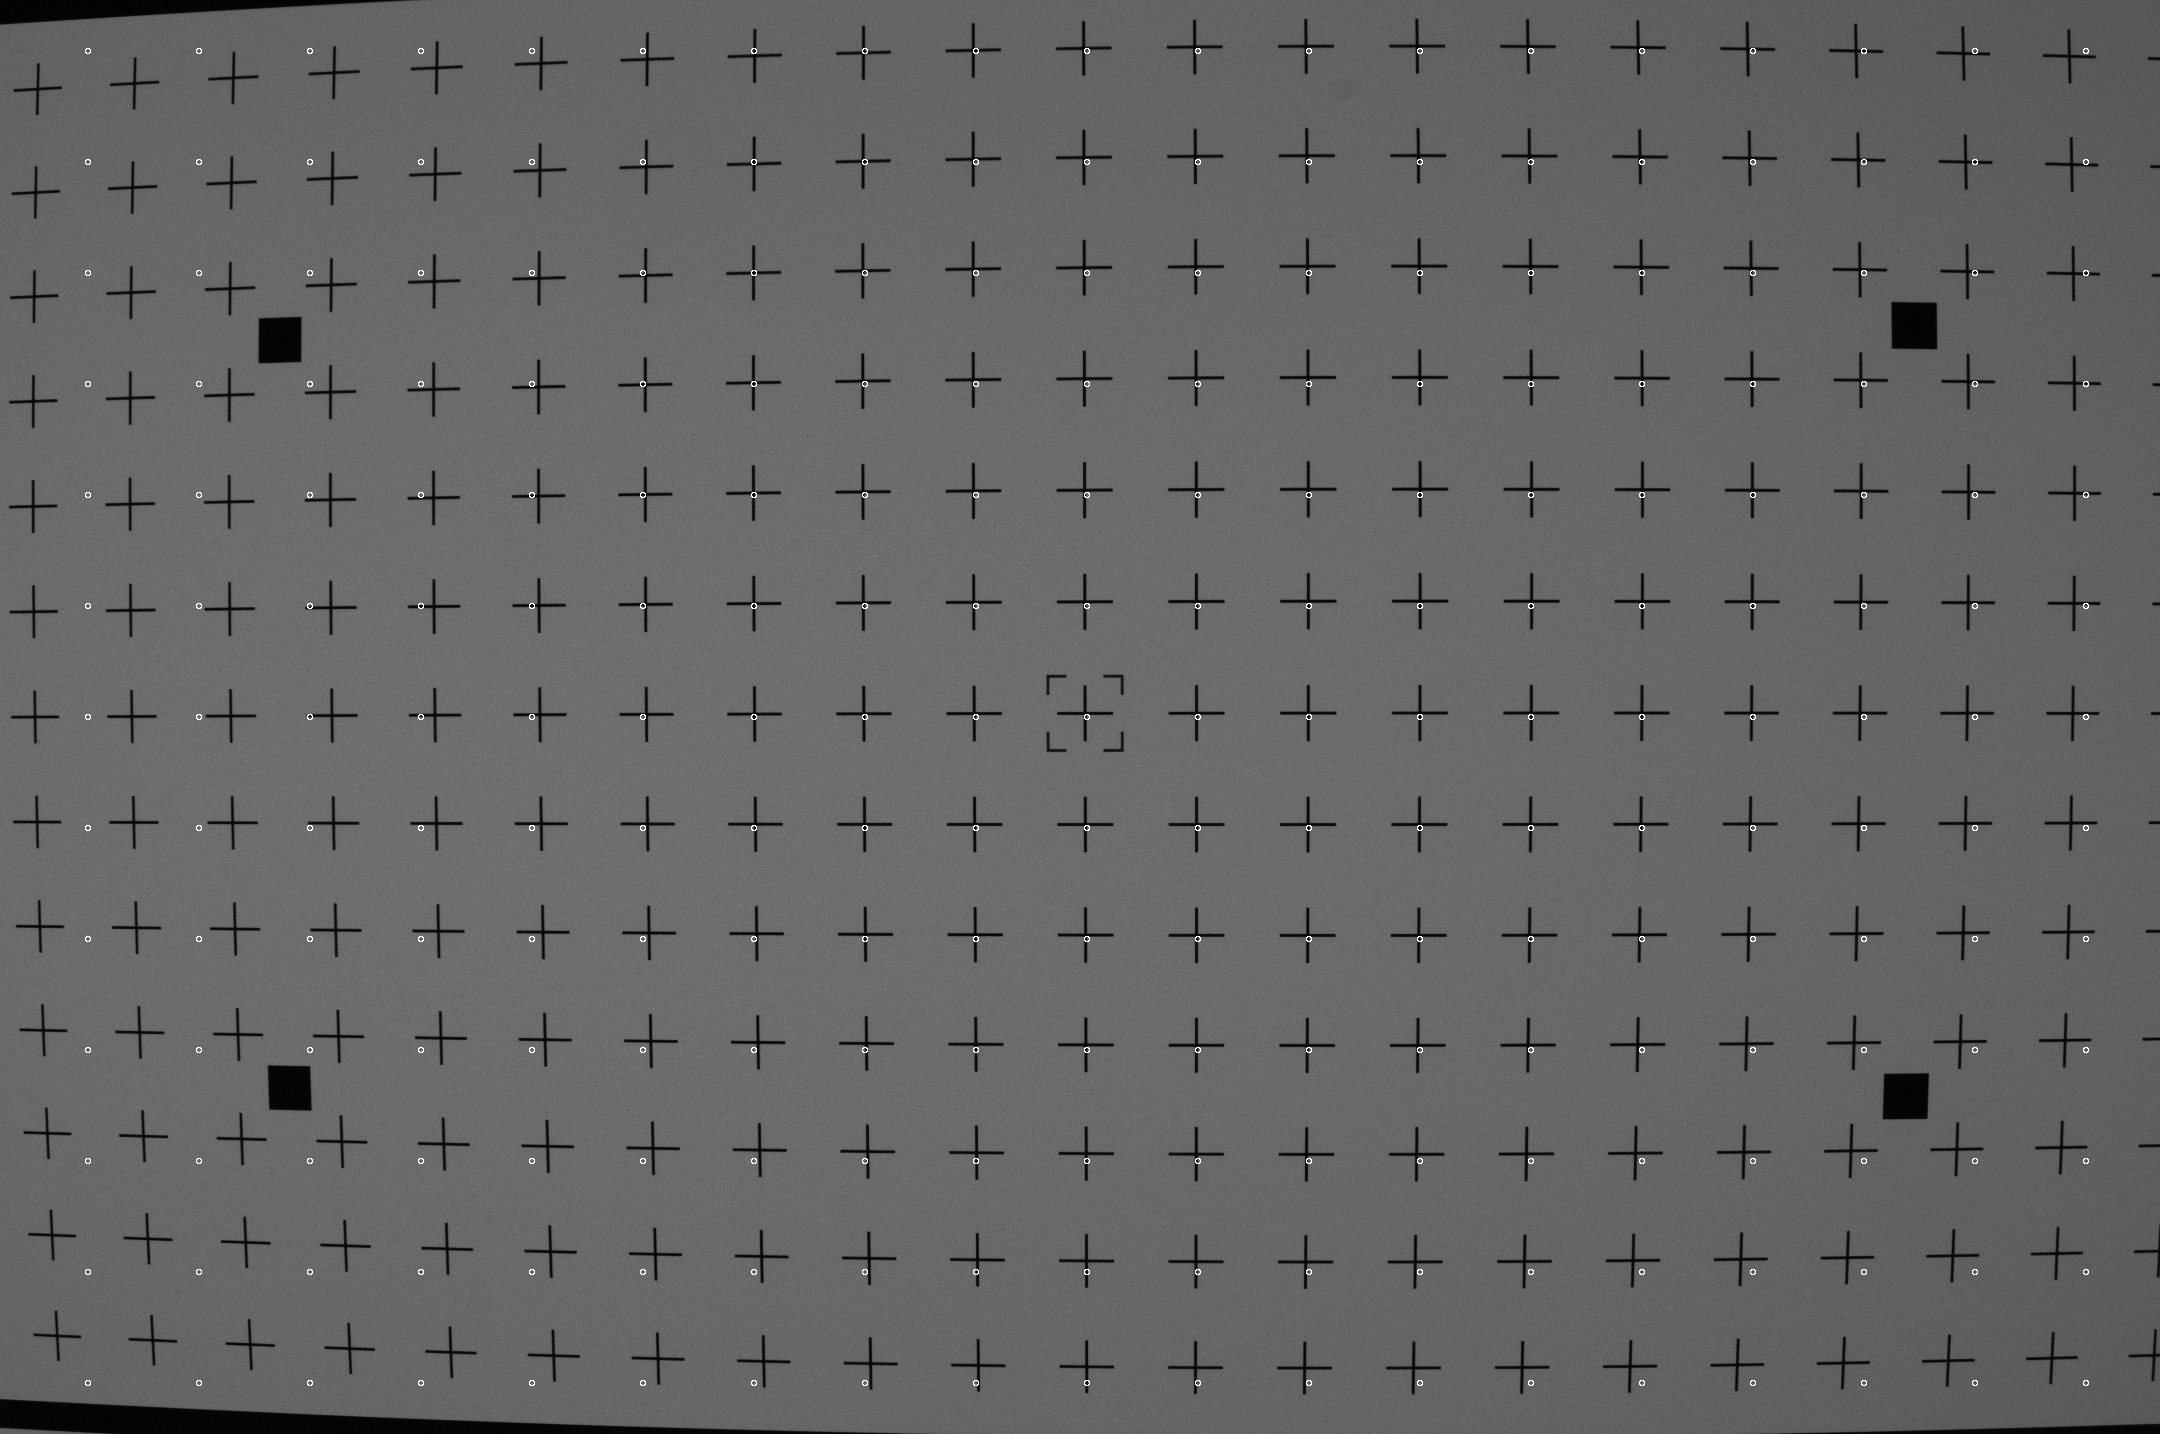
\includegraphics[width=\textwidth]{Images/optimales-gitter.png}
\caption{Erzeugte Zielpunkte mit Hilfe der $compute\_draw\_optimal\_Grid()$ Methode}
\label{fig:gitter-optimal}
\end{figure}

\subsection{Aufstellung des Problems}
\label{sec:Problem}

In Formel~\ref{equ:Levenberg} wird das Modell der LMA definiert und in Formel~\ref{equ:RDF} die RDF angeben. 
Für den Ausgleich eines radial verzerrten Bildes muss zunächst das entsprechende Modell für die RDF definiert werden. Zunächst wird die Matrix $F(x) \in \mathbb{R}^M$ mit $x = \begin{pmatrix}
\kappa_1 & \kappa_2 & \kappa_3\end{pmatrix}^T$ laut Formel~\ref{equ:Problem} aufgestellt. Wie bereits in Abschnitt~\ref{sec:RDF} erwähnt wird aus nummerischen Gründen die Form $r^2$ verwendet, welche den Rundungsfehler und den Rechenaufwand minimiert. 

\todo[inline, color=red]{Vera: $r^2$ ersetzen}

\begin{equation}
\label{equ:Problem}
\begin{aligned}
&F(x)=
\begin{pmatrix}
(1+\kappa_1 r + \kappa_2 r^2 + \kappa_3 r^3)d_x^0 -u_x^0\\
(1+\kappa_1 r + \kappa_2 r^2 + \kappa_3 r^3)d_y^0 -u_y^0\\
(1+\kappa_1 r + \kappa_2 r^2 + \kappa_3 r^3)d_x^i -u_x^i\\
(1+\kappa_1 r + \kappa_2 r^2 + \kappa_3 r^3)d_y^i -u_y^i\\
\vdots\\
(1+\kappa_1 r + \kappa_2 r^2 + \kappa_3 r^3)d_x^M -u_x^M\\
(1+\kappa_1 r + \kappa_2 r^2 + \kappa_3 r^3)d_y^M -u_y^M\\
\end{pmatrix}
&mit\ i = 0,\dots,M
\end{aligned}
\end{equation}

Die benötigte Jacobi-Matrix $F'(x)$ ergibt sich aus der Definition in Formel~\ref{equ:Jacobi} .

\begin{equation}
\label{equ:Jacobi}
\begin{aligned}
&F'(x)=
\begin{pmatrix}
\frac{\delta F_0}{\delta \kappa_1} & \frac{\delta F_0}{\delta \kappa_2} & \frac{\delta F_0}{\delta \kappa_2}\\
\frac{\delta F_1}{\delta \kappa_1} & \frac{\delta F_1}{\delta \kappa_2} & \frac{\delta F_1}{\delta \kappa_2}\\
 \vdots & \vdots & \vdots \\
\frac{\delta F_M}{\delta \kappa_1} & \frac{\delta F_M}{\delta \kappa_2} & \frac{\delta F_M}{\delta \kappa_2}\\
\end{pmatrix}= \begin{pmatrix}
rd_x^0 & r^2d_x^0 & r^3d_x^0\\
rd_y^0 & r^2d_y^0 & r^3d_y^0\\
rd_x^1 & r^2d_x^i & r^3d_x^i\\
rd_y^1 & r^2d_y^i & r^3d_y^i\\
\vdots & \vdots & \vdots \\
rd_x^M & r^2d_x^M & r^3d_x^M\\
rd_y^M & r^2d_y^M & r^3d_y^M\\
\end{pmatrix}
&mit\ i = 0,\dots,M
\end{aligned}
\end{equation}

\subsection{Initialisierung des Minimierungsverfahren}
\label{sec:Minimierung}
Das Minimierungsverfahren wird unter anderem mit dem Vektor $F(x)$ und der korrespondierenden Jacobi-Matrix $F'(x)$ initialisiert. Anderes als bei der Problemaufstellung in Abschnitt~\ref{sec:Problem} wird für die Intialisierung ein weiterer Vektor $t \in \mathbb{R}^M$, wie in Formel~\ref{equ:Stuetzstellen}, eingeführt. Dieser Vektor enthält alle idealen Punktraster-Koordinaten $u^i$. Darum entfallen folglich in $F(x)$ alle $u_x^i$ und $u_y^i$.
\begin{equation}
\label{equ:Stuetzstellen}
\begin{aligned}
&t(u)=
\begin{pmatrix}
u_x^0&
u_y^0&
u_x^i&
u_y^i&
\dots&
u_x^M&
u_y^M&
\end{pmatrix}^T
&mit\ i = 0,\dots,M
\end{aligned}
\end{equation}
Der Startvektor $x_0$ wird mit Koeffizienten initialisiert die keine Verzerrung beschreiben. Es gilt also für $x_0 = \begin{pmatrix}
0 & 0 & 0
\end{pmatrix}^T$. Zur Beschränkung der Rechenzeit des Optimierers wird die maximale Anzahl von Iterationen auf $500$ und die maximale Anzahl von Rechenschritten auf den doppelten Wert festgelegt.

%@Vera: vorher stand da das:
%Um unnötigen Rechenaufwand wird die maximale Anzahl von Iterationen auf $500$ und die maximale Anzahl von Rechenschritten auf den doppelten Wert festgelegt.

\subsection{Plugin-Klassen}
\label{sec:PluginKlassen}

Im folgenden werden die Methoden der einzelnen Klassen erläutert. Die vollständige UML zur besseren Verständlichkeit der Klassenbeziehungen ist der Abbildung~\ref{img:UML} zu entnehmen.

\begin{figure}[H] %muss gesetzt werden sonnst rutscht das bild in ein anderes kapitel
	\center
	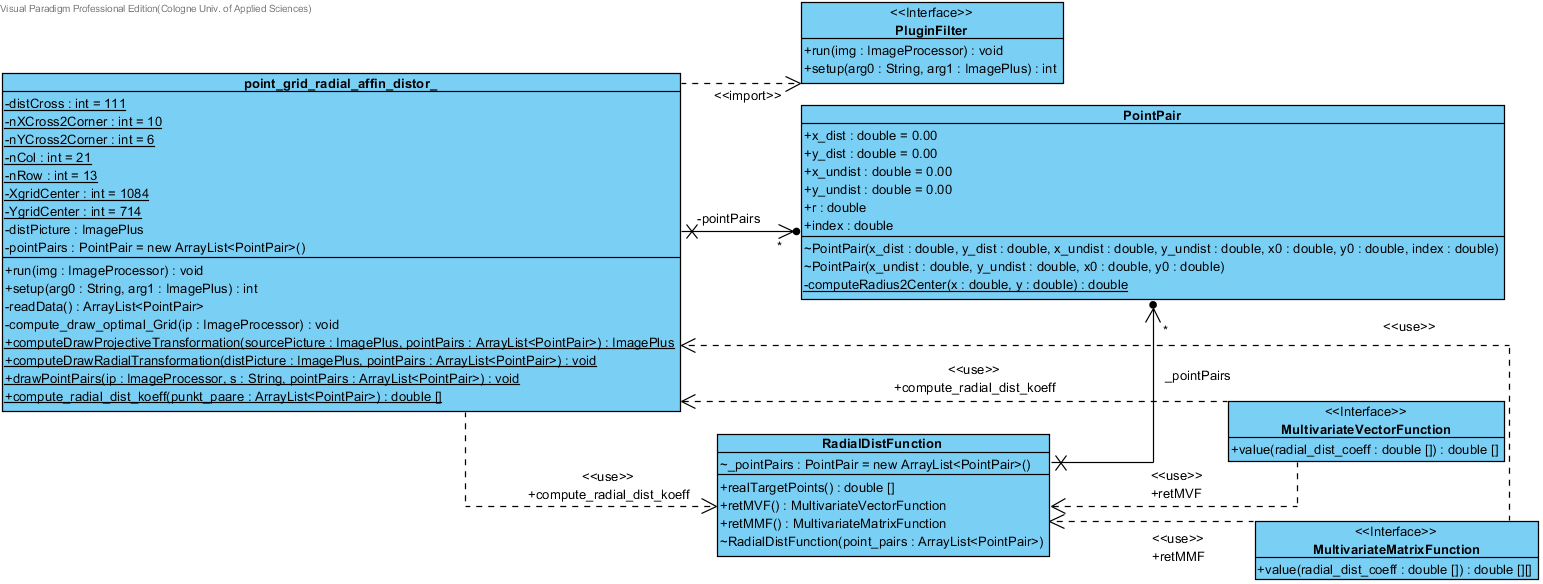
\includegraphics[width=\textheight, angle =90]{Images/Class Diagram1.png}
	\caption{UML Klassendiagramm}
	\label{img:UML}
\end{figure}

\subsubsection{point\_grid\_radial\_affin\_distor\_}
Hauptklasse der Anwendung. Implementiert das Interface \texttt{PluginFilter} um über ImageJ aufgerufen werden zu können.

Die Klasse besitzt folgende Methoden und deren Funktion:

\begin{table}[H]
	\begin{tabular}{|p{0.45\textwidth} | p{0.55\textwidth}|} 
		\hline
		\texttt{run()} & Main-Methode des PlugIns in der die Optimierung aufgerufen wird\\ \hline
		\texttt{setup()} & Konstruktor-Methode des PlugIns mit der die Bildreferenz abgespeichert wird\\ \hline
		\texttt{compute\_draw\_optimal\_Grid()} & Berechnung und Abbildung des optimalen Gitters anhand der Klassenkonstanten \\ \hline
		\texttt{readData()} & Liest aus einer in ImageJ geöffneten UnwarpJ-Landmarks Datei Punkt-Paare ein für die Start- und Ziel-Koordinaten\\\hline
		\texttt{computeDrawRadial Transformation()} & Startet die Berechnung der radialen Verzerrung und zeichnet das dazugehörige entzerrte Bild\\ \hline
		\texttt{computeDrawProjective Transformation()} & Berechnet anhand von Punkpaaren die projektive Transformation und gibt die Abbildung zurück. Zusätzlich werden die Punkt-Paare mit transformiert.\\ \hline
		\texttt{drawTargets()} & Zeichnet Punkte an den übergebenen Start- und Ziel-Koordinaten in das übergebene Bild\\ \hline
		\texttt{compute\_radial\_dist\_koeff()} & Berechnet mit dem Levenberg-Marquadt Optimierer die Koeffizienten der radialen Verzerrung der übergebenen Punkte und gibt die Koeffizienten zurück\\ 
		\hline
	\end{tabular}
	\caption{Methoden der \texttt{point\_grid\_radial\_affin\_distor\_} Klasse}
\end{table}

\subsubsection{PointPair}
Eine einfache Klasse zum Speichern der Vorgabe- und Ziel- Koordinaten und des Abstandes zum Mittelpunkt. Sie besitzt einen Konstruktor bei dem der Mittelpunktabstand anhand der Parameter automatisch berechnet und gespeichert wird. Dies ist nützlich, da so der Radius nicht in einem externen Aufruf berechnet werden muss.

\subsubsection{RadialDistFunction}
Klasse zum Erzeugen der Funktionen für den Levenber-Marquadt-Optimierer~\cite{optimizer_example}. Die Klasse besitzt folgende Methoden:

\begin{table}[H]
	\begin{tabular}{|p{0.45\textwidth} | p{0.55\textwidth}|} 
		\hline
		\texttt{RadialDistFunction()} & Konstruktor der Klasse. Es wird ein \texttt{PointPair} Array erwartet welcher Koordinaten-Paare für Start- und Ziel-Koordinaten enthält.\\ \hline
		\texttt{realTargetPoints()} & Gibt ein Array aus welches nur die Ziel-Koordinaten enthält. Dieses wird für den Optimierer benötigt.\\ \hline
		\texttt{retMVF()} & Funktion zur Modellierung der Radialen Verzerrung für den Optimierer. Berechnet zu den Vorgegeben Koeffizienten und einer Start-Koordinate die Ziel-Koordinate\\ \hline
		\texttt{retMMF()} & Jacobi-Matrix-Funktion zur Berechnung der Ableitung nach den einzelnen vom Optimierer vorgegebenen Koeffizienten \\ 
		\hline
	\end{tabular}
	\caption{Methoden der \texttt{RadialDistFunction} Klasse}
\end{table}

